\section{Security \& Compliance}\label{sec:security-&-compliace}

\subsection{Shared Responsibility Model}\label{subsec:shared-responsibility-model}

\begin{enumerate}
    \item{\textbf{AWS Responsibility:} Security \textbf{of} the cloud}.
        Protecting infrastructure (hw, software, facilities and networking).
    \item{\textbf{Customer Responsibility:} Security \textbf{in} the cloud}.
        Depends on the service, example EC2, customer is responsible for managing guest OS, IAM, firewall
        and network config.
    \item{\textbf{Shared controls:} Patch management, configuration management, awareness and training.}
\end{enumerate}

\begin{figure}[h]
    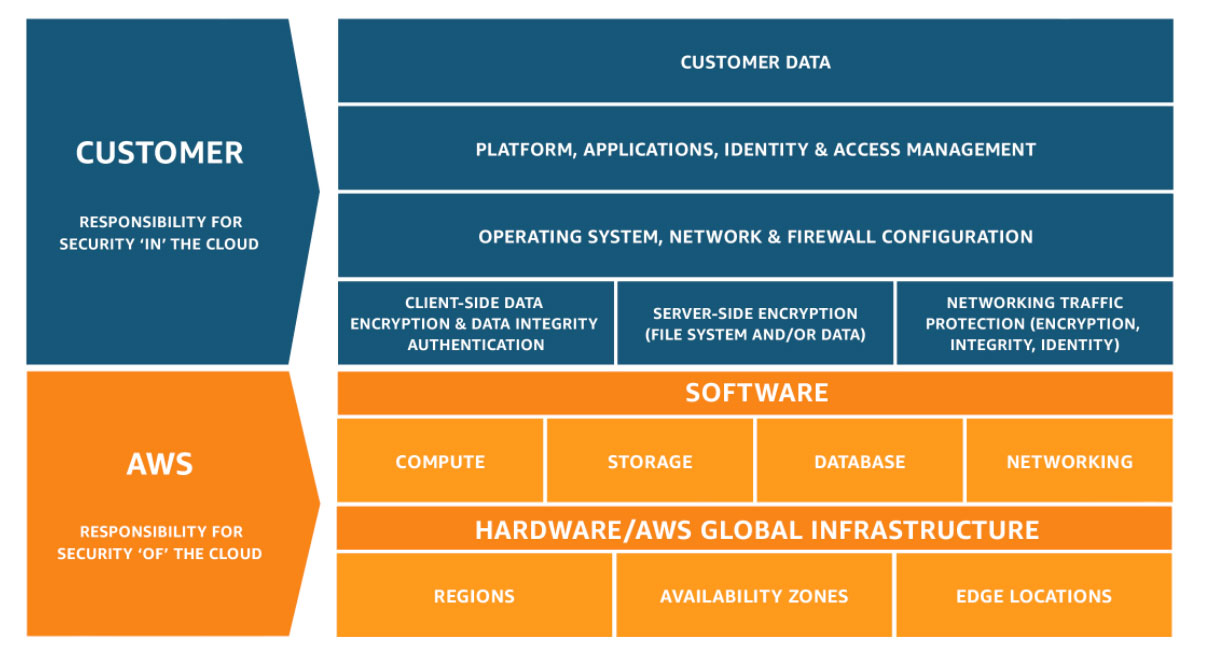
\includegraphics[scale=0.30]{security-compliance/shared-reponsibility-model}
    \centering
    \label{fig:shared-reponsibility-model}
\end{figure}

\subsection{Shield}\label{subsec:shield}

\begin{itemize}
    \item{\textbf{Shield Standard:}} (Free)
        \begin{itemize}
            \item{Provides protection within 3rd \& 4th OSI Layer (attacks such as SYN/UDP Flood, Reflection Attack)}
        \end{itemize}
    \item{\textbf{Shield Advanced:}} (Expensive ~\$3K/mo per org.)
        \begin{itemize}
            \item{Provides more sophisticated protection on EC2, ELB, Cloudfront, Global Accelerator, Route 53}
            \item{24/7 access to AWS DDoS reponse team}
            \item{Protect against high fees during usage skipe due to DDoS}
        \end{itemize}
\end{itemize}

\subsection{WAF}\label{subsec:waf}

\begin{itemize}
    \item{Protects agains common web (OSI Layer 7) exploits}
    \item{Deploys on ALB, API Gateway, CloudFront}
    \item{Define Web ACL (Web Access Control List)}
\end{itemize}

\subsection{Network Firewall}\label{subsec:network-firewall}

\begin{itemize}
    \item{Define firewall rules and provides fine-grain control over network traffic}
    \item{Protects your entire VPC (From Layer 3 to Layer 7)}
\end{itemize}

\subsection{Pen Testing}\label{subsec:pen-testing}

In a nutshell, you can pen-test this services (but there's a catch):

\begin{itemize}
    \item{EC2}
    \item{NAT gateway}
    \item{Load Balancer}
    \item{RDS}
    \item{Cloudfront}
    \item{Aurora}
    \item{API Gateway}
    \item{Lambda \& Lambda Edge function}
    \item{Lightsail}
    \item{Elastic Beanstalk}
\end{itemize}

But you cannot perform some activities:

\begin{itemize}
    \item{DNS zone walking in Amazon Route53}
    \item{DoS, DDoS, Simulated Dos, Simulated DDoS}
    \item{Port flooding}
    \item{Protocol flooding}
    \item{Request flooding}
\end{itemize}

\subsection{KMS encryption \& Cloud HSM}\label{subsec:kms-encryption-&-cloud-hsm}

This encryption can be:

\begin{itemize}
    \item{\textbf{Data at rest:} Data stored or archived (Hard Disk, RDS, S3, etc)}
    \item{\textbf{Data in transit:} Data in motion (transfered on the network)}
\end{itemize}

KMS (Key Management Service) manages the keys used for encryption.

CloudHSM (Hardware Security Module) provision encryption dedicated hardware.

Types of KMS keys:

\begin{itemize}
    \item{\textbf{Customer Managed:} Create, manage and used by customer (can enable o disable). Can bring your own key}
    \item{\textbf{AWS Managed:} Created, managed and used on customer's behalf by AWS}
    \item{\textbf{AWS Owned:} AWS itself owns and manages it, and use for internal AWS services protection.}
    \item{\textbf{CloudHSM Keys:} Created from your own CLoudHSM hardware device.}
\end{itemize}

\subsection{ACM}\label{subsec:acm}

ACM (AWS Certificate Manager) enable the provision, management and deployment of SSL/TLS Certificates.
It integrates with ELB, CloudFront, API Gateway.

\subsection{Secrets Manager}\label{subsec:secrets-manager}

Service for storing secrets, with rotation capabilities using KMS\.

\subsection{Artifact}\label{subsec:artifact}

Portal that provides customers with on-demand access to AWS compliance (ISO, PCI, SOC) documentation and
AWS agreements (BAA, HIPAA).

\subsection{GuardDuty}\label{subsec:guardduty}

Service that uses ML to discover and protect your AWS account.
It discovers anomalies from: CloudTrail logs, VPC logs, DNS logs, etc.

\subsection{Inspector}\label{subsec:inspector}

Service that performs automated security assessments for:

\begin{itemize}
    \item{\textbf{EC2:} It uses SSM (System Manager) to analyze for known vulnerabilities.}
    \item{\textbf{ECR:} Assesses the image as they are pushed.}
    \item{\textbf{Lambda:} Identifies vulnerabilities in code and package deps.}
\end{itemize}


\subsection{Config}\label{subsec:config}

Helps record configurations and changes of AWS services overtime.
The config can be stored into S3.

\subsection{Macie}\label{subsec:macie}

Fully managed service that uses ML to discover and protect sensitive data in AWS\.
Helps identify sensitive data, such as personally identifiable information (PII).

\subsection{Security Hub}\label{subsec:security-hub}
